\chapter{Methodology}
\label{ch:method}

\section{Algorithms description}
The algorithms essential for forest fire prediction, ranging from traditional regression to advanced ensemble methods, vital for understanding their roles in our study.
\begin{itemize}

\item Linear Regression

Linear regression is a simple and fast algorithm used for regression analysis. It models the relationship between a dependent variable and one or more independent variables by fitting a linear
equation to observed data points.

\item SVM Regressor

Support Vector Machine (SVM) regressor is a supervised learning algorithm used for regression tasks. It works by finding the hyperplane that best fits the data while maximizing the margin
between different classes.

\item Decision Tree Regressor

Decision tree regressor is a non-parametric supervised learning method used for regression tasks. It recursively splits the data into subsets based on the value of a chosen feature to predict the target variable.

\item Random Forest Regressor

Random Forest regressor is an ensemble learning method that constructs multiple decision trees during training and outputs the average prediction of the individual trees.

\item Extra Tree Regressor

Extra Tree regressor is another ensemble learning method similar to Random Forests but with slightly different tree construction methods.

\item XGBoost

XGBoost is a scalable and efficient gradient boosting library that is widely used for regression and classification tasks. It builds multiple decision trees iteratively and combines their predictions to improve accuracy.

\item LightGBM

LightGBM is a gradient boosting framework developed by Microsoft that focuses on leaf-wise tree growth and gradient-based learning. It is known for its high efficiency and performance.

\item Em CatBoost
CatBoost is a gradient boosting library developed by Yandex that is designed to handle categorical features automatically. It is known for its robustness and ability to work with heterogeneous data
\end{itemize}


\section{Tables}
Data types of each column in the DataFrame df \\
\begin{table}[ht!]
    \centering
    \begin{tabular}{ c c }
 X          & int64 \\
 Y          & int64 \\ 
 month     & object \\ 
 day       & object \\ 
 FFMC     & float64 \\
 DMC      & float64 \\
 DC       & float64 \\
 ISI      & float64 \\
 temp     & float64 \\
 RH       & int64 \\
 wind     & float64 \\
 rain     & float64 \\
 target   & float64 \\
\end{tabular}
    \label{tab:Datatypes}
    \caption{Data types of each column in the DataFrame df}
\end{table}

\clearpage
\section{Code}
Code snippet in LATEX and this is a Python code example
\begin{lstlisting}
from ucimlrepo import fetch_ucirepo
import numpy np
import pandas pd
forest_fires = fetch_ucirepo(id=162)
X = forest_fires.data.features
Y = forest_fires.data.targets
df = pd.DataFrame(data=X, columns=forest_fires.feature_names)
df['target'] = Y
print(forest_fires.metadata)

print(forest_fires.variables)

print(df.head(10))

print("Statistical Description:", df.describe())

print("Data Types:", df.dtypes)

print("Correlation:", df.corr(method='pearson'))
import matplotlib.pyplot as plt
plt.figure(figsize=(6.5, 6.5))
df['target'].hist()
plt.title('Histogram of Target Column')
plt.xlabel('Target Values')
plt.ylabel('Frequency')
plt.show()
n_cols = len(df.columns)
layout = (n_cols // 2, 2)
plt.figure(figsize=(6.5, 6.5))
df.hist(layout=layout, figsize=(6.5, 6.5))
plt.tight_layout()
plt.show()
import numpy as np
fig, ax = plt.subplots(figsize=(6.5, 6.5))
cax = ax.matshow(df.corr(), vmin=-1, vmax=1)
fig.colorbar(cax)
ticks = np.arange(0, len(df.columns), 1)
ax.set_xticks(ticks)
ax.set_yticks(ticks)
ax.set_xticklabels(df.columns, rotation=45, ha='left')
ax.set_yticklabels(df.columns)
plt.show()
import matplotlib.pyplot as plt
plt.figure(figsize=(6.5, 6.5))
sns.barplot(x='month', y='target', data=df)
plt.title('Average Target by Month')
plt.xlabel('Month')
plt.ylabel('Average Target')
plt.show()
\end{lstlisting}

\clearpage
First 10 rows of Data frame
\begin{table}[ht!]
    \centering
    \section{Tables}
\begin{tabular}{ |c|c|c|c|c|c|c|c|c|c|c|c|c|c| }
\hline
& X & Y & month & day & FFMC & DMC & DC & ISI & temp & RH & wind & rain & target \\
0 & 7 & 5 & mar & fri & 86.2 & 26.2 & 94.3 & 5.1 & 8.2 & 51 & 6.7 & 0.0 & 0.0 \\
1 & 7 & 4 & oct & tue & 90.6 & 35.4 & 669.1 & 6.7 & 18.0 & 33 & 0.9 & 0.0 & 0.0 \\
2 & 7 & 4 & oct & sat & 90.6 & 43.7 & 686.9 & 6.7 & 14.6 & 33 & 1.3 & 0.0 & 0.0 \\
3 & 8 & 6 & mar & fri & 91.7 & 33.3 & 77.5  & 9.0 &  8.3 & 97 & 4.0 & 0.2 & 0.0 \\
4 & 8 & 6 & mar & sun & 89.3 & 51.3 & 102.2 & 9.6 & 11.4 & 99 & 1.8 & 0.0 & 0.0 \\
5 & 8 & 6 & aug & sun & 92.3 & 85.3 & 488.0 & 14.7 & 22.2 & 29 & 5.4 & 0.0 & 0.0 \\
6 & 8 & 6 & aug & mon & 92.3 & 88.9 & 495.6 & 8.5 & 24.1 & 27 & 3.1 & 0.0 & 0.0 \\
7 & 8 & 6 & aug & mon & 91.5 & 145.4 & 608.2 & 10.7 & 8.0 & 86 & 2.2 & 0.0 & 0.0 \\
8 & 8 & 6 & sep & tue & 91.0 & 129.5 & 692.6 & 7.0 & 13.1 & 63 & 5.4 & 0.0 & 0.0 \\
9 & 7 & 5 & sep & sat & 92.5 &  88.0 & 698.6 & 7.1 & 22.8 & 40 & 4.0 & 0.0 & 0.0 \\
\hline
\end{tabular}
    \label{tab:DataFrame}
    \caption{First 10 rows of Data frame}
\end{table}

\clearpage
\section{Figure}
\begin{figure}[ht]
    \centering
    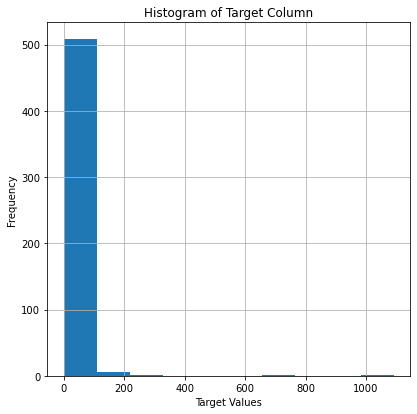
\includegraphics[scale=1.0]{figures/output_14_0.png}
    \caption{Histogram representation of Target column and Frequency.}
    \label{fig:example-01}
\end{figure}
\clearpage
Histograms for each column in the DataFrame using a specified layout
\begin{figure}[ht]
    \centering
    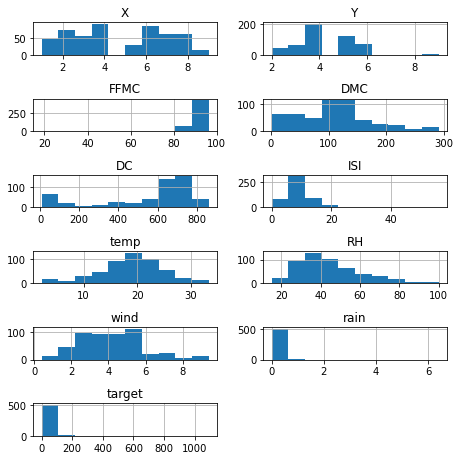
\includegraphics[scale=1.0]{figures/output_16_1.png}
    \caption{Histograms for each column in the DataFrame using a specified layout.}
    \label{fig:example-01}
\end{figure}

\clearpage
Bar plot showing the average target value for each month
\begin{figure}[ht]
    \centering
    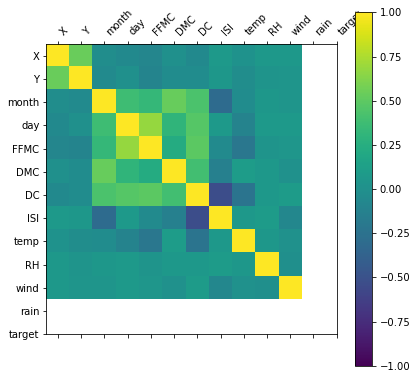
\includegraphics[scale=1.0]{figures/output_18_0.png}
    \caption{Bar plot showing the average target value for each month.}
    \label{fig:example-01}
\end{figure}

\clearpage
\section {Implementation}
During our implementation phase, we strategically utilized XGBoost, known for its speed, accuracy,and advanced features such as regularization, parallelization, and feature importance scoring. 

This algorithm proved beneficial for balanced datasets incorporating both numerical and categorical features, as well as projects necessitating extensive documentation and community support.

LightGBM, renowned for its training speed, memory efficiency, and proficiency with large datasets, was a natural choice for scenarios with vast data volumes and concerns about overfitting. 

CatBoost, tailored for categorical features and imbalanced data, emerged as the preferred option for datasets characterized by categorical dominance and class imbalances, as well as projects seeking
efficient default settings and enhanced interpretability.

\section {Experiments Design}
\begin{itemize}
\item Data Collection:
A dataset consisting of meteorological and other relevant variables from the northeast region of Portugal was collected for training and evaluating the models. This dataset includes features such as
temperature, humidity, wind speed, and precipitation, along with historical records of forest fire occurrences.

\item Model Training and Evaluation:
The collected data was split into training and testing sets for model training and evaluation respectively. Cross-validation techniques such as k-fold cross-validation were employed to assess
the models' performance robustly. Various metrics including mean squared error (MSE), root mean squared error (RMSE), and R-squared score (R2) were used to evaluate the models' performance.

\item Feature Importance Analysis:
The importance of features in predicting the target variable (area or skewed area) was analyzed using techniques such as permutation importance or feature importance scores provided by the models. This analysis helps in identifying the most influential features for predicting forest fire area.

\item Comparison of Top Dependable Variables vs. All Variables:
The performance of the models using only the top 5 dependable columns versus using all columns was compared to assess the impact of feature selection on prediction accuracy.
\end{itemize}

\section {Summary}
In this methodology, we described the algorithms employed in our study, including traditional regression algorithms and gradient boosting algorithms. These algorithms were implemented using Python, and experiments were conducted on a dataset from Portugal to predict forest fire occurrences. The models were trained and evaluated using appropriate techniques, and the results were analyzed to provide insights into the effectiveness of the prediction methodologies. Additionally, feature importance analysis was performed to identify the most significant predictors of forest fire area. Comparison between top 5 dependable columns and all columns is conducted to understand the impact of feature selection on model performance.